\documentclass[fontsize=12pt,
               paper=a4,
               twoside=false,
               parskip=half,
               ]{scrartcl}

% Load the packages
% Packages Template
% =================
% 
% Contains packages used for project documentation
% 
% @author burgc5
% 
% To use this simply enter: % Packages Template
% =================
% 
% Contains packages used for project documentation
% 
% @author burgc5
% 
% To use this simply enter: % Packages Template
% =================
% 
% Contains packages used for project documentation
% 
% @author burgc5
% 
% To use this simply enter: \input{./packages.tex}

\usepackage[utf8]{inputenc}
\usepackage[T1]{fontenc}

% Set font to latin modern
\usepackage{lmodern}

\usepackage[pdftex]{graphicx}
\usepackage{epstopdf}

% Create links in pdf documents
\usepackage[colorlinks,pdfpagelabels,pdfstartview=FitH,bookmarksopen=true,bookmarksnumbered=true,linkcolor=black,plainpages=false,hypertexnames=false,citecolor=black] {hyperref}
\hypersetup{
    colorlinks,%
    citecolor=black,%
    filecolor=black,%
    linkcolor=black,%
    urlcolor=black
}
\urlstyle{same}

% Use \enquote{} to create quotation marks
\usepackage{csquotes}

% Create professional tables with booktabs
% @see http://en.wikibooks.org/wiki/LaTeX/Tables#Professional_tables
\usepackage{booktabs}

% Customizable enumerates/itemizes
\usepackage{enumitem}

% SVN meta information
\usepackage{svn}


\usepackage[utf8]{inputenc}
\usepackage[T1]{fontenc}

% Set font to latin modern
\usepackage{lmodern}

\usepackage[pdftex]{graphicx}
\usepackage{epstopdf}

% Create links in pdf documents
\usepackage[colorlinks,pdfpagelabels,pdfstartview=FitH,bookmarksopen=true,bookmarksnumbered=true,linkcolor=black,plainpages=false,hypertexnames=false,citecolor=black] {hyperref}
\hypersetup{
    colorlinks,%
    citecolor=black,%
    filecolor=black,%
    linkcolor=black,%
    urlcolor=black
}
\urlstyle{same}

% Use \enquote{} to create quotation marks
\usepackage{csquotes}

% Create professional tables with booktabs
% @see http://en.wikibooks.org/wiki/LaTeX/Tables#Professional_tables
\usepackage{booktabs}

% Customizable enumerates/itemizes
\usepackage{enumitem}

% SVN meta information
\usepackage{svn}


\usepackage[utf8]{inputenc}
\usepackage[T1]{fontenc}

% Set font to latin modern
\usepackage{lmodern}

\usepackage[pdftex]{graphicx}
\usepackage{epstopdf}

% Create links in pdf documents
\usepackage[colorlinks,pdfpagelabels,pdfstartview=FitH,bookmarksopen=true,bookmarksnumbered=true,linkcolor=black,plainpages=false,hypertexnames=false,citecolor=black] {hyperref}
\hypersetup{
    colorlinks,%
    citecolor=black,%
    filecolor=black,%
    linkcolor=black,%
    urlcolor=black
}
\urlstyle{same}

% Use \enquote{} to create quotation marks
\usepackage{csquotes}

% Create professional tables with booktabs
% @see http://en.wikibooks.org/wiki/LaTeX/Tables#Professional_tables
\usepackage{booktabs}

% Customizable enumerates/itemizes
\usepackage{enumitem}

% SVN meta information
\usepackage{svn}


% SVN Meta
\SVN $Date: 2012-05-13 23:59:53 +0200 (So, 13 Mai 2012) $
\SVN $Revision: 123 $
\SVN $HeadURL: https://svn.bfh.ch/repos/projects/patmon1/trunk/doc/src/design_model.tex $


\begin{document}

% Document title for title.tex
\newcommand{\doctitle}{Design Model}
% Titlepage Template
% ==================
% 
% @author burgc5
% 
% To use this simply enter: % Titlepage Template
% ==================
% 
% @author burgc5
% 
% To use this simply enter: % Titlepage Template
% ==================
% 
% @author burgc5
% 
% To use this simply enter: \input{./title.tex}
% 
% You have to define the commands '\doctitle' and '\docrevision' to give the 
% document a title and a revision on its titlepage.
% Do this with the following command:
% \newcommand{\doctitle}{Document title goes here}
%
% SVN:
% ----
% You also have to define the variables:
% \SVN $Date$
% \SVN $Revision$
%
% As executing the following command on the file:
% > svn propset svn:keywords "Date Revision" filename.tex
% 
% This titlepage needs:
% \usepackage[pdftex]{graphicx}
% \usepackage{svn}
%

\begin{titlepage}

\begin{center}

% Team-logo
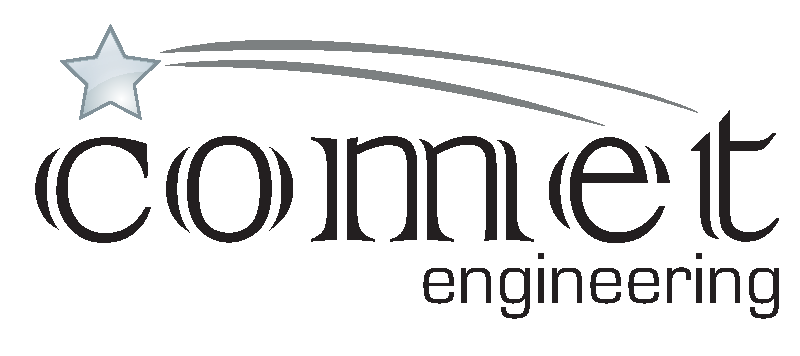
\includegraphics[width=0.35\textwidth]{./comet-logo.eps}\\[2.5cm]    

% Project title
\textsc{\Large Comet Patient Monitor}\\[2cm]

% Document title
{ \huge \bfseries \doctitle{}}\\[3cm]

% Members/Client
\begin{minipage}{0.45\textwidth}
\begin{flushleft} \large
\emph{Team Members:}\\
Patrick \textsc{Haring}\\
Christian \textsc{Bürgi}
\end{flushleft}
\end{minipage}
\begin{minipage}{0.45\textwidth}
\begin{flushright} \large
\emph{Client:} \\
Prof.~Dr.~Olivier \textsc{Biberstein}\\
~
\end{flushright}
\end{minipage}

\vfill

{\large 
Revision: \SVNRevision \\[0.2cm]
\SVNDate \\[0.2cm]
{\footnotesize \itshape \url{\SVNHeadURL?p=\SVNRevision}}}

\end{center}

\end{titlepage}
% 
% You have to define the commands '\doctitle' and '\docrevision' to give the 
% document a title and a revision on its titlepage.
% Do this with the following command:
% \newcommand{\doctitle}{Document title goes here}
%
% SVN:
% ----
% You also have to define the variables:
% \SVN $Date$
% \SVN $Revision$
%
% As executing the following command on the file:
% > svn propset svn:keywords "Date Revision" filename.tex
% 
% This titlepage needs:
% \usepackage[pdftex]{graphicx}
% \usepackage{svn}
%

\begin{titlepage}

\begin{center}

% Team-logo
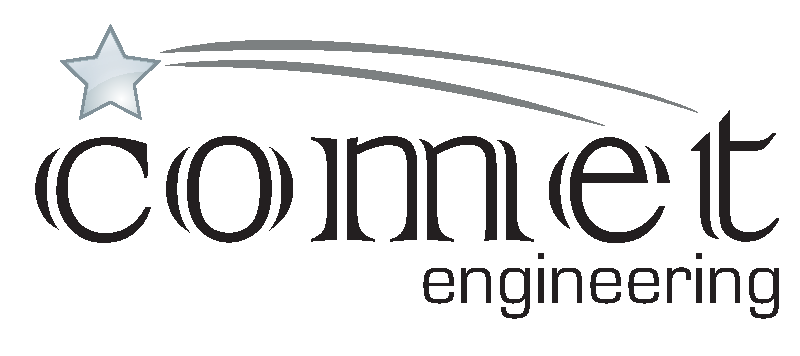
\includegraphics[width=0.35\textwidth]{./comet-logo.eps}\\[2.5cm]    

% Project title
\textsc{\Large Comet Patient Monitor}\\[2cm]

% Document title
{ \huge \bfseries \doctitle{}}\\[3cm]

% Members/Client
\begin{minipage}{0.45\textwidth}
\begin{flushleft} \large
\emph{Team Members:}\\
Patrick \textsc{Haring}\\
Christian \textsc{Bürgi}
\end{flushleft}
\end{minipage}
\begin{minipage}{0.45\textwidth}
\begin{flushright} \large
\emph{Client:} \\
Prof.~Dr.~Olivier \textsc{Biberstein}\\
~
\end{flushright}
\end{minipage}

\vfill

{\large 
Revision: \SVNRevision \\[0.2cm]
\SVNDate \\[0.2cm]
{\footnotesize \itshape \url{\SVNHeadURL?p=\SVNRevision}}}

\end{center}

\end{titlepage}
% 
% You have to define the commands '\doctitle' and '\docrevision' to give the 
% document a title and a revision on its titlepage.
% Do this with the following command:
% \newcommand{\doctitle}{Document title goes here}
%
% SVN:
% ----
% You also have to define the variables:
% \SVN $Date$
% \SVN $Revision$
%
% As executing the following command on the file:
% > svn propset svn:keywords "Date Revision" filename.tex
% 
% This titlepage needs:
% \usepackage[pdftex]{graphicx}
% \usepackage{svn}
%

\begin{titlepage}

\begin{center}

% Team-logo
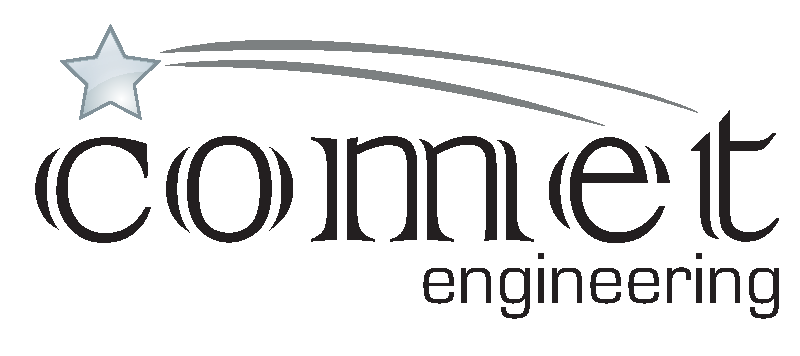
\includegraphics[width=0.35\textwidth]{./comet-logo.eps}\\[2.5cm]    

% Project title
\textsc{\Large Comet Patient Monitor}\\[2cm]

% Document title
{ \huge \bfseries \doctitle{}}\\[3cm]

% Members/Client
\begin{minipage}{0.45\textwidth}
\begin{flushleft} \large
\emph{Team Members:}\\
Patrick \textsc{Haring}\\
Christian \textsc{Bürgi}
\end{flushleft}
\end{minipage}
\begin{minipage}{0.45\textwidth}
\begin{flushright} \large
\emph{Client:} \\
Prof.~Dr.~Olivier \textsc{Biberstein}\\
~
\end{flushright}
\end{minipage}

\vfill

{\large 
Revision: \SVNRevision \\[0.2cm]
\SVNDate \\[0.2cm]
{\footnotesize \itshape \url{\SVNHeadURL?p=\SVNRevision}}}

\end{center}

\end{titlepage}

\tableofcontents


% ====
% SSDs
% ====

\section{Doctor login}

\subsection{System sequence diagram}

% Diagram generated with astah
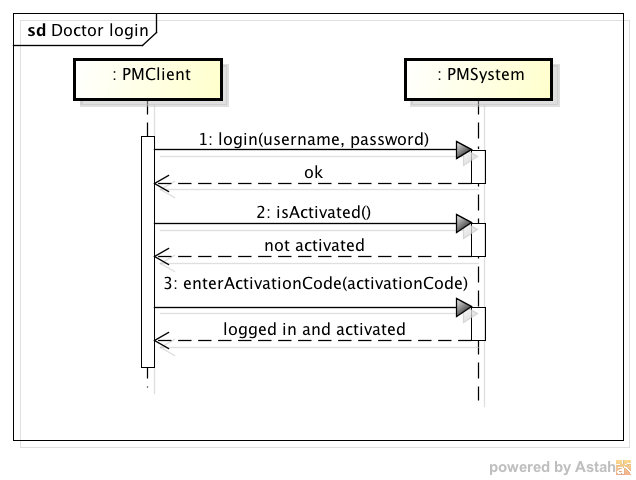
\includegraphics[width=10cm]{./img/system-sequence-diagrams/doctor-login.png}

This diagram describes the communication between the client and the server during a login of a doctor. The client sends a login message containing the login information of the doctor. The server confirms and then the client follows protocol checking if the account doctor is activated and proceeds with activating the doctor.

\subsection{Sequence diagram}

% Diagram generated with astah
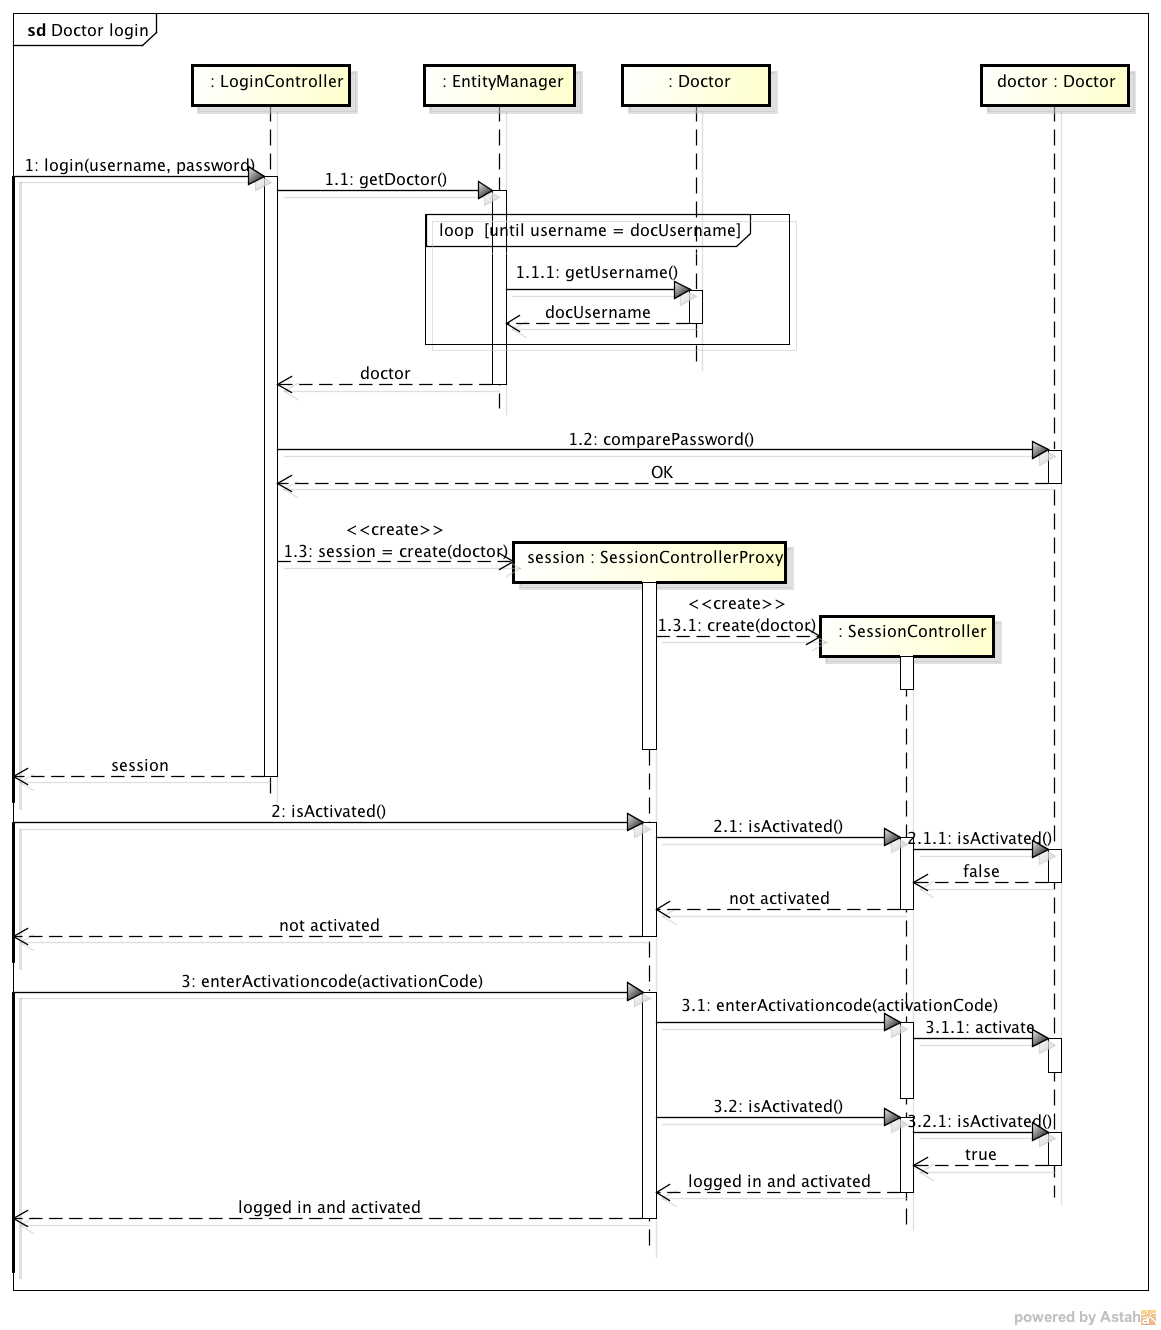
\includegraphics[width=15cm]{./img/sequence-diagrams/doctor-login.png}

There is a login controller for all doctor login messages. It looks up the doctor using the entity manager and lets the doctor (if found) check the credentials. If this succeeds, a session controller is created, which is responsible for the current session of the client. For security reasons, there is also a proxy for the controller which is sent to the client instead of the controller itself. The client then checks activation and activates the login via the session controller.

\subsection{Design class diagram}

% Diagram generated with astah
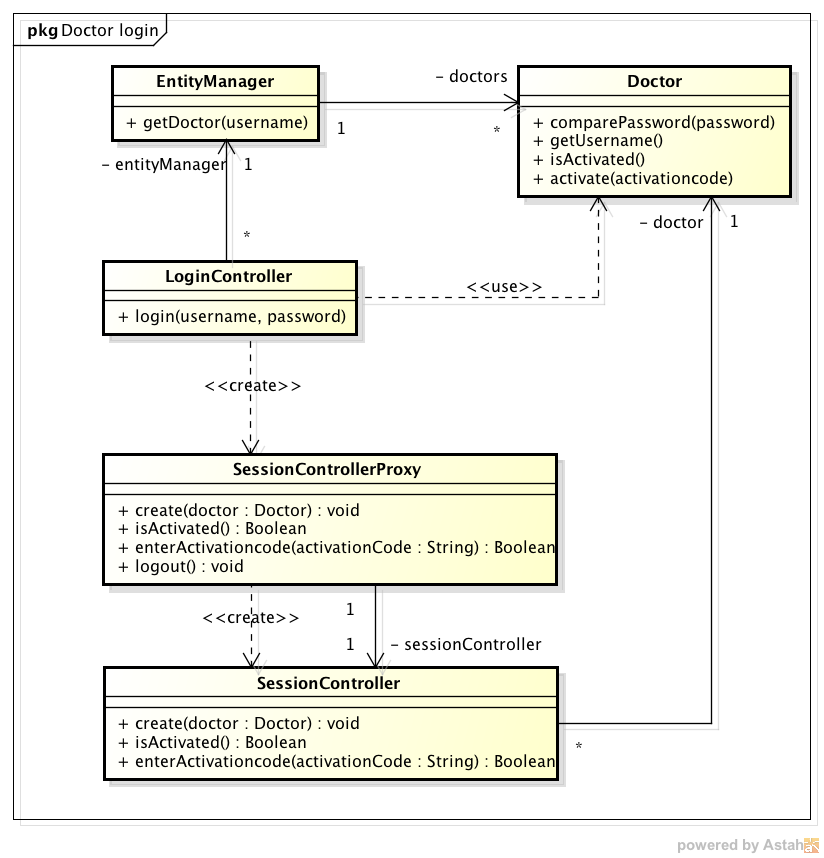
\includegraphics[width=15cm]{./img/design-class-diagrams/doctor-login.png}

Thesession controller gets access to the doctor using the entity manager. After creating the session controller, the doctor is referenced by the session controller.

\section{Logout}

\subsection{System sequence diagram}

% Diagram generated with astah
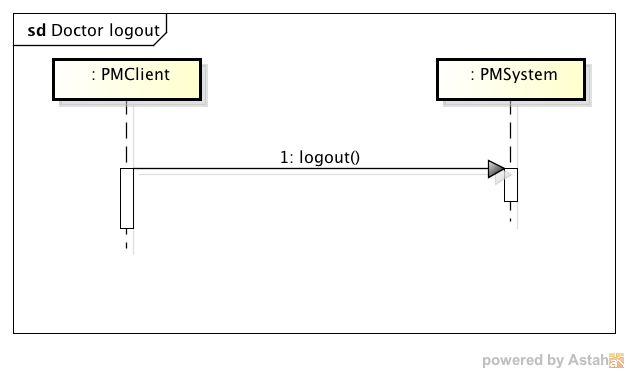
\includegraphics[width=10cm]{./img/system-sequence-diagrams/doctor-logout.png}

A logout is done simply by sending a logout message from the client to the server.

\subsection{Sequence diagram}

% Diagram generated with astah
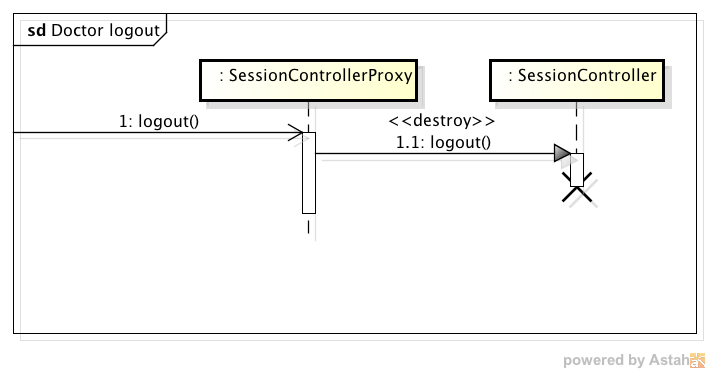
\includegraphics[width=10cm]{./img/sequence-diagrams/doctor-logout.png}

A logout on the session controller proxy destroys the session controller. Because the session controller only lives on the server, there is no way for the client to sent messages to the server, because he only has a reference to the proxy.

\subsection{Design class diagram}

% Diagram generated with astah
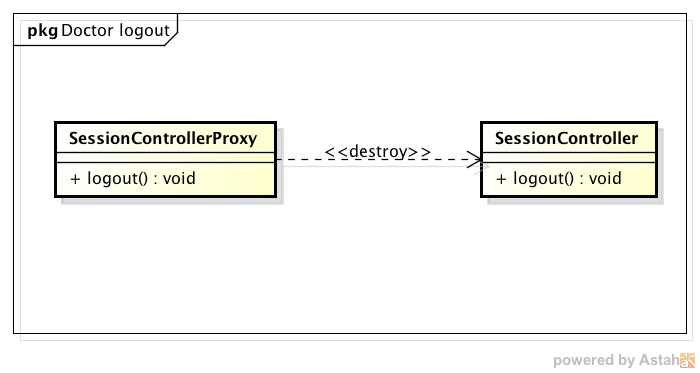
\includegraphics[width=8cm]{./img/design-class-diagrams/doctor-logout.png}

During logout the proxy destroys the session controller.

\section{Register patient}

\subsection{System sequence diagram}

% Diagram generated with astah
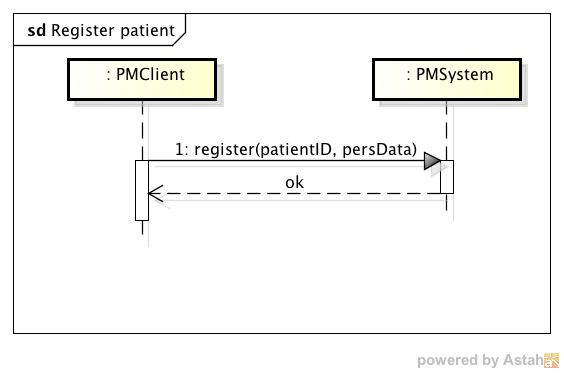
\includegraphics[width=10cm]{./img/system-sequence-diagrams/register-patient.png}

The diagram shows the communication between the client and the patient monitoring system. The client sends the patients SSN as the patientID and adds the personal data. If the registration went well the System will send a confirmation signal.


\subsection{Sequence diagram}

% Diagram generated with astah
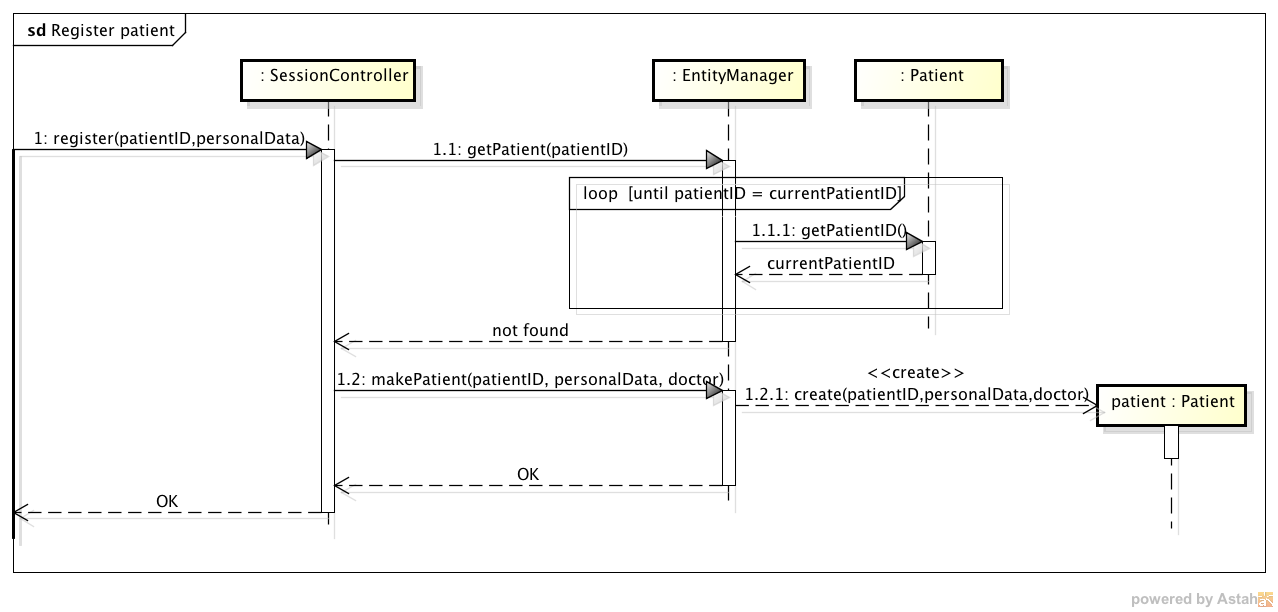
\includegraphics[width=15cm]{./img/sequence-diagrams/register-patient.png}

The SessionController looks up if the patients id (his SSN) was already registered in the system and if not e will create a new patient by calling the makePatient method of the EntitiyManager.

\subsection{Design class diagram}

% Diagram generated with astah
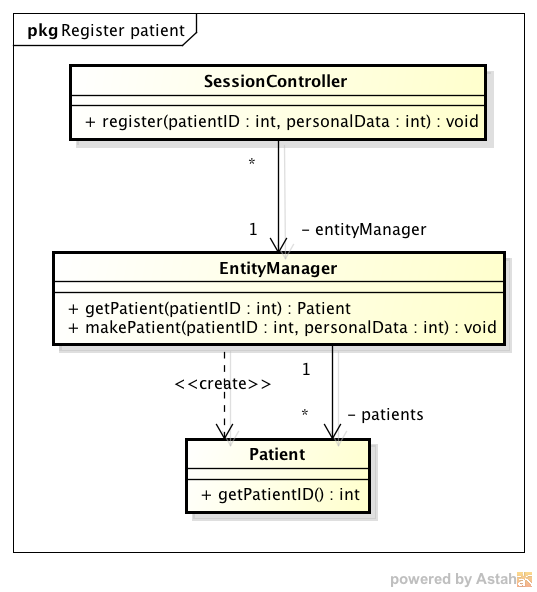
\includegraphics[width=10cm]{./img/design-class-diagrams/register-patient.png}

The SessionController creates a new patient via the the makePatient method of the EntityManager.

\section{Define observation period}

\subsection{System sequence diagram}

% Diagram generated with astah
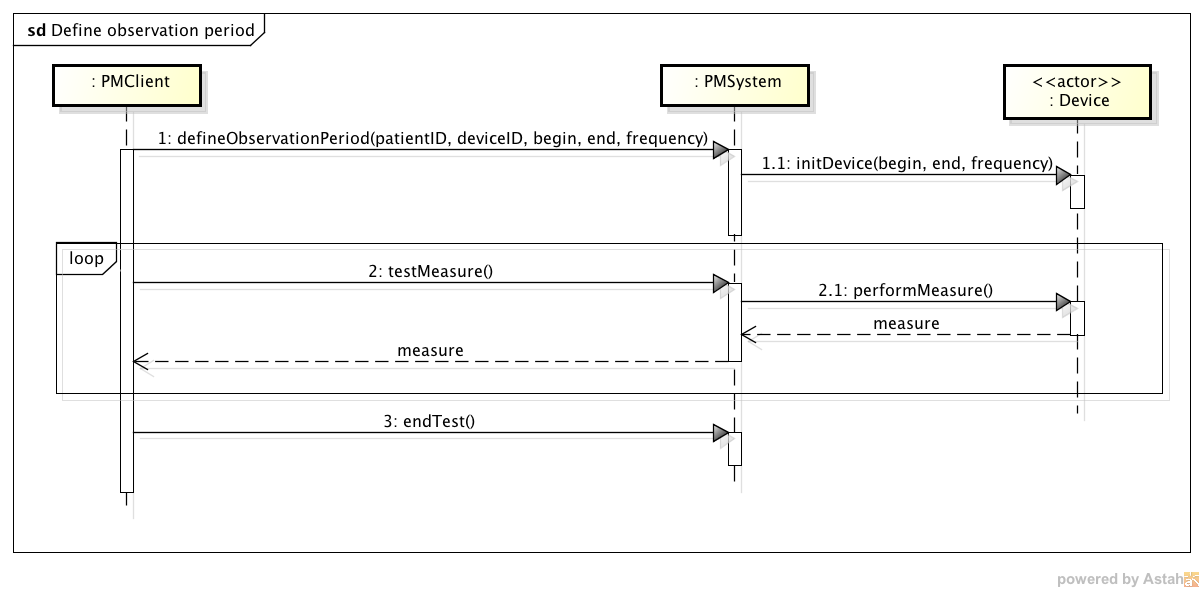
\includegraphics[width=15cm]{./img/system-sequence-diagrams/define-observation-period.png}

For defining an observation period, the client sends a message to the server. After this, the device is initialized with the data of the period. Then the client performs test-measures by sending a message to the server. The system itself sends a performMeasure-message to the device which performs a measure and sends it to the system. This procedure can be repeated multiple times and is ended with an endTest-message.

\subsection{Sequence diagram}

% Diagram generated with astah
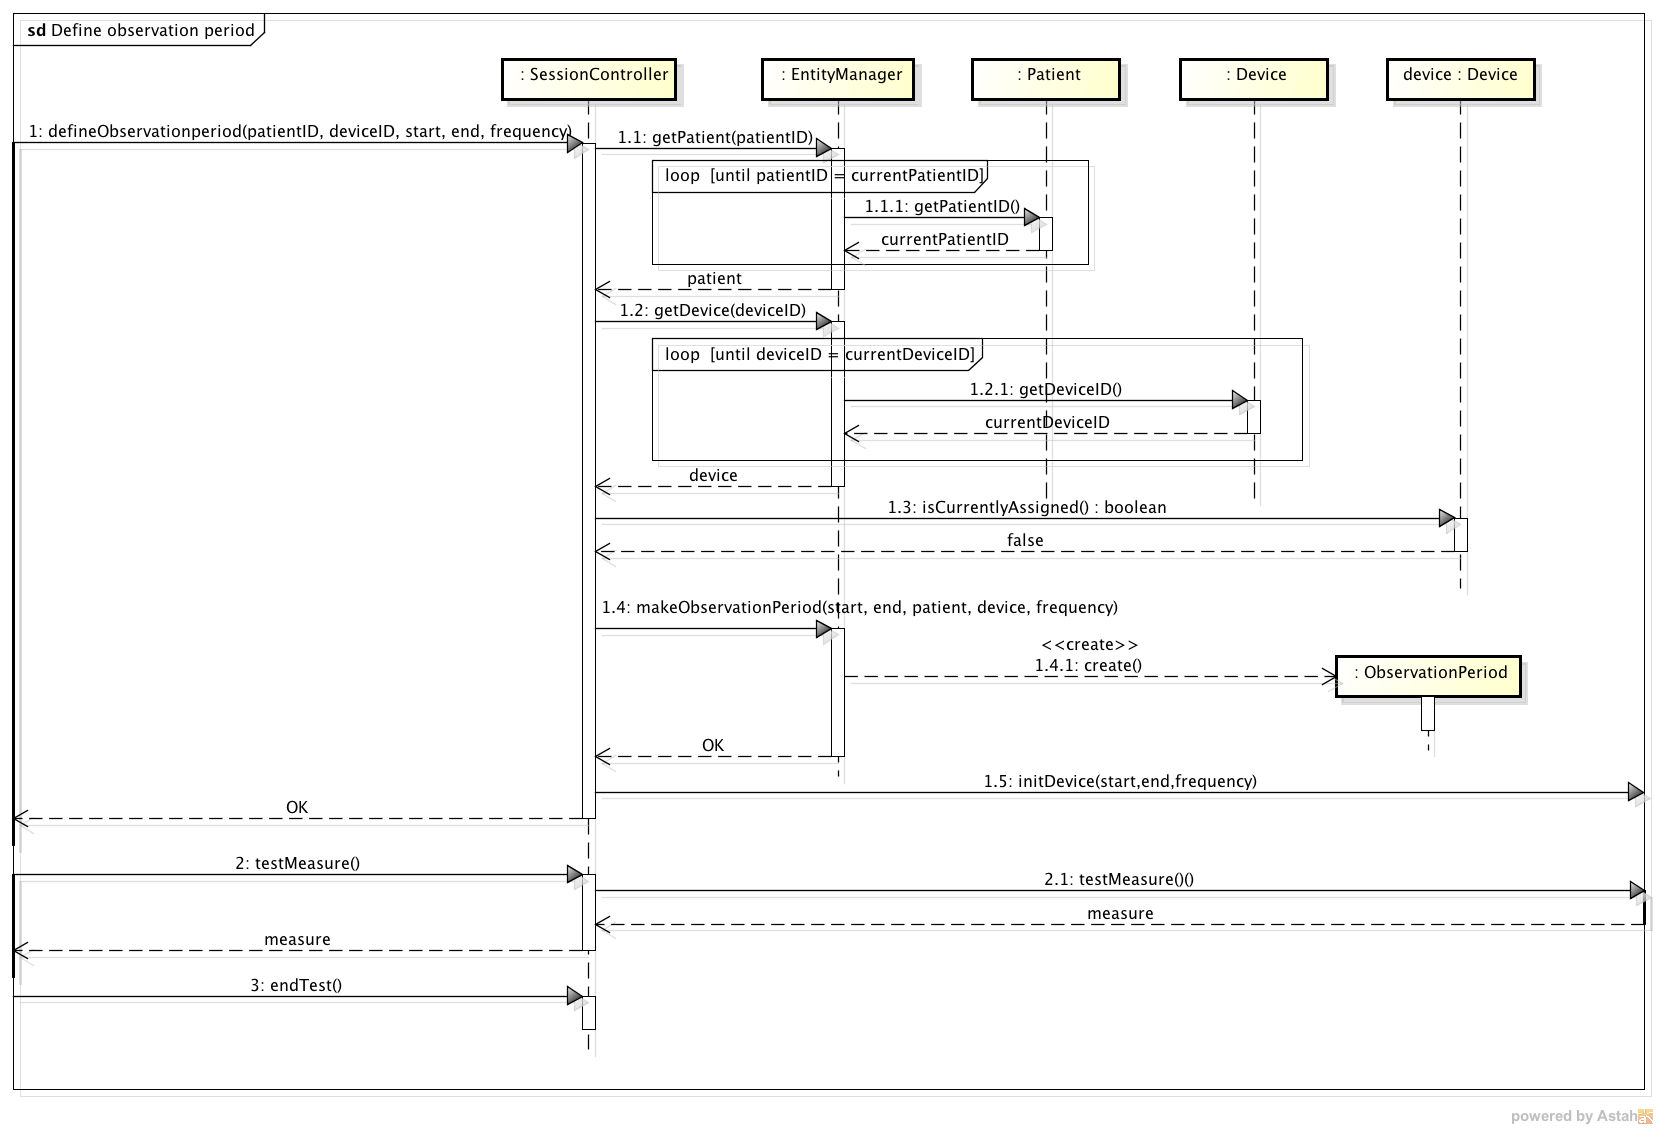
\includegraphics[width=15cm]{./img/sequence-diagrams/define-observation-period.png}

For defining an observation period, the session controller gets the patient and device from the entity manager. Then it creates an observation period using the entity manager.

\subsection{Design class diagram}

% Diagram generated with astah
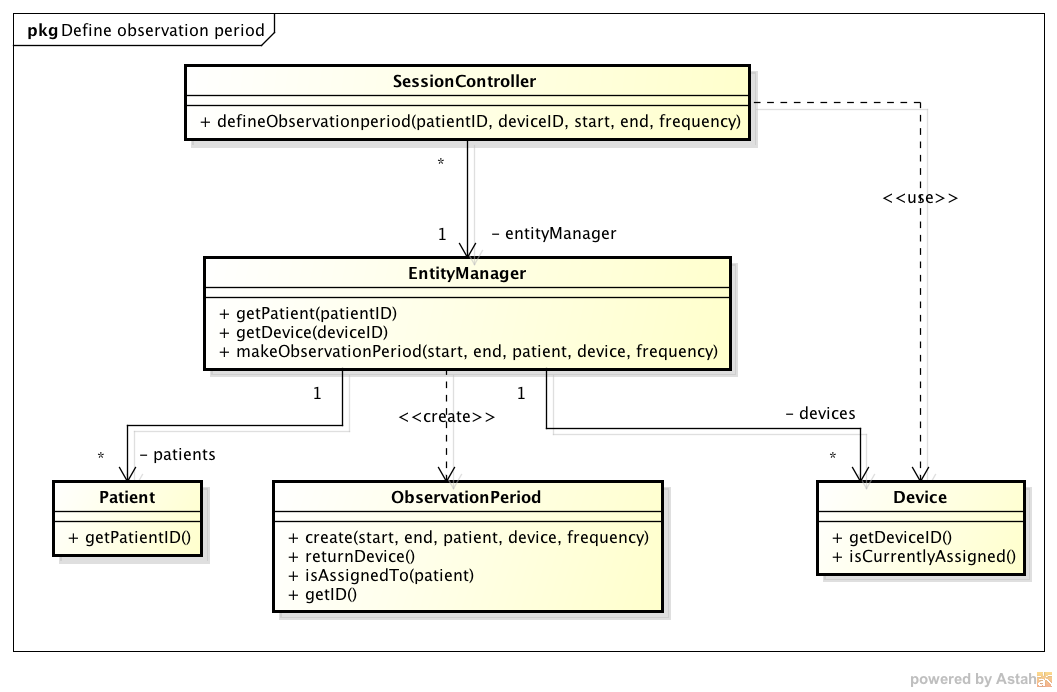
\includegraphics[width=15cm]{./img/design-class-diagrams/define-observation-period.png}

The session controller gets patient and device from the entity manager and lets it create an observation period.

\section{Consult measurements}

\subsection{System sequence diagram}

% Diagram generated with astah
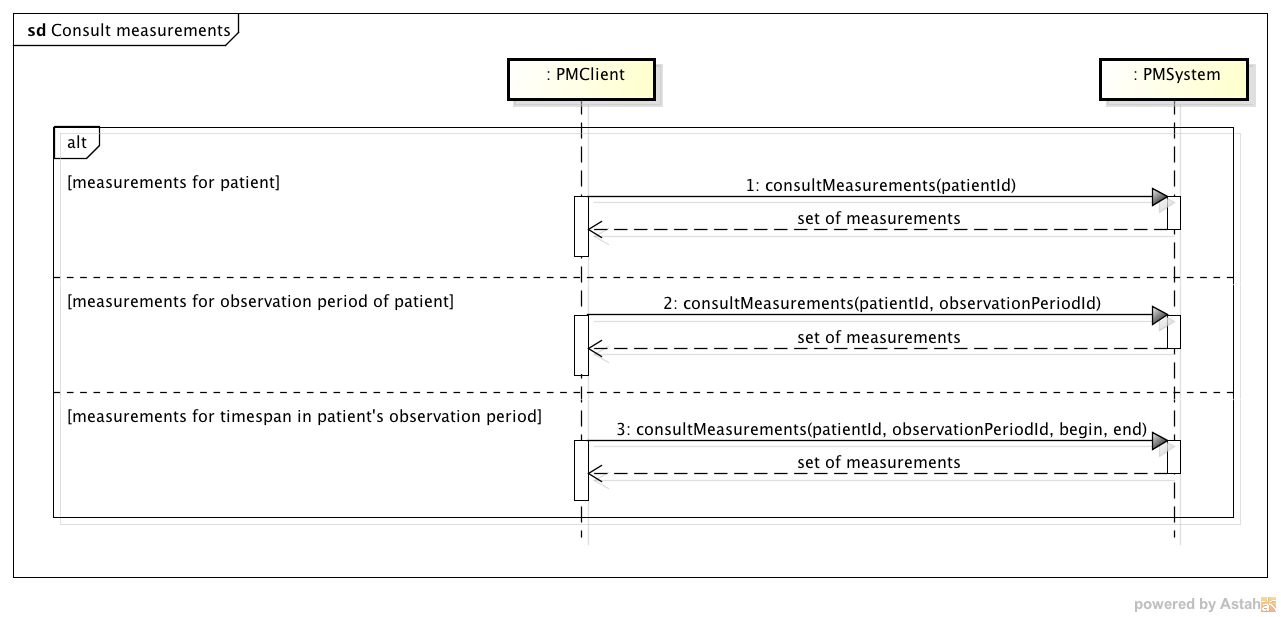
\includegraphics[width=15cm]{./img/system-sequence-diagrams/consult-measurements.png}

There are three different ways of querying data which apply to this use case. We can implement the most difficult one and implement the others by setting the parameters in the right manner.

\subsection{Sequence diagram}

% Diagram generated with astah
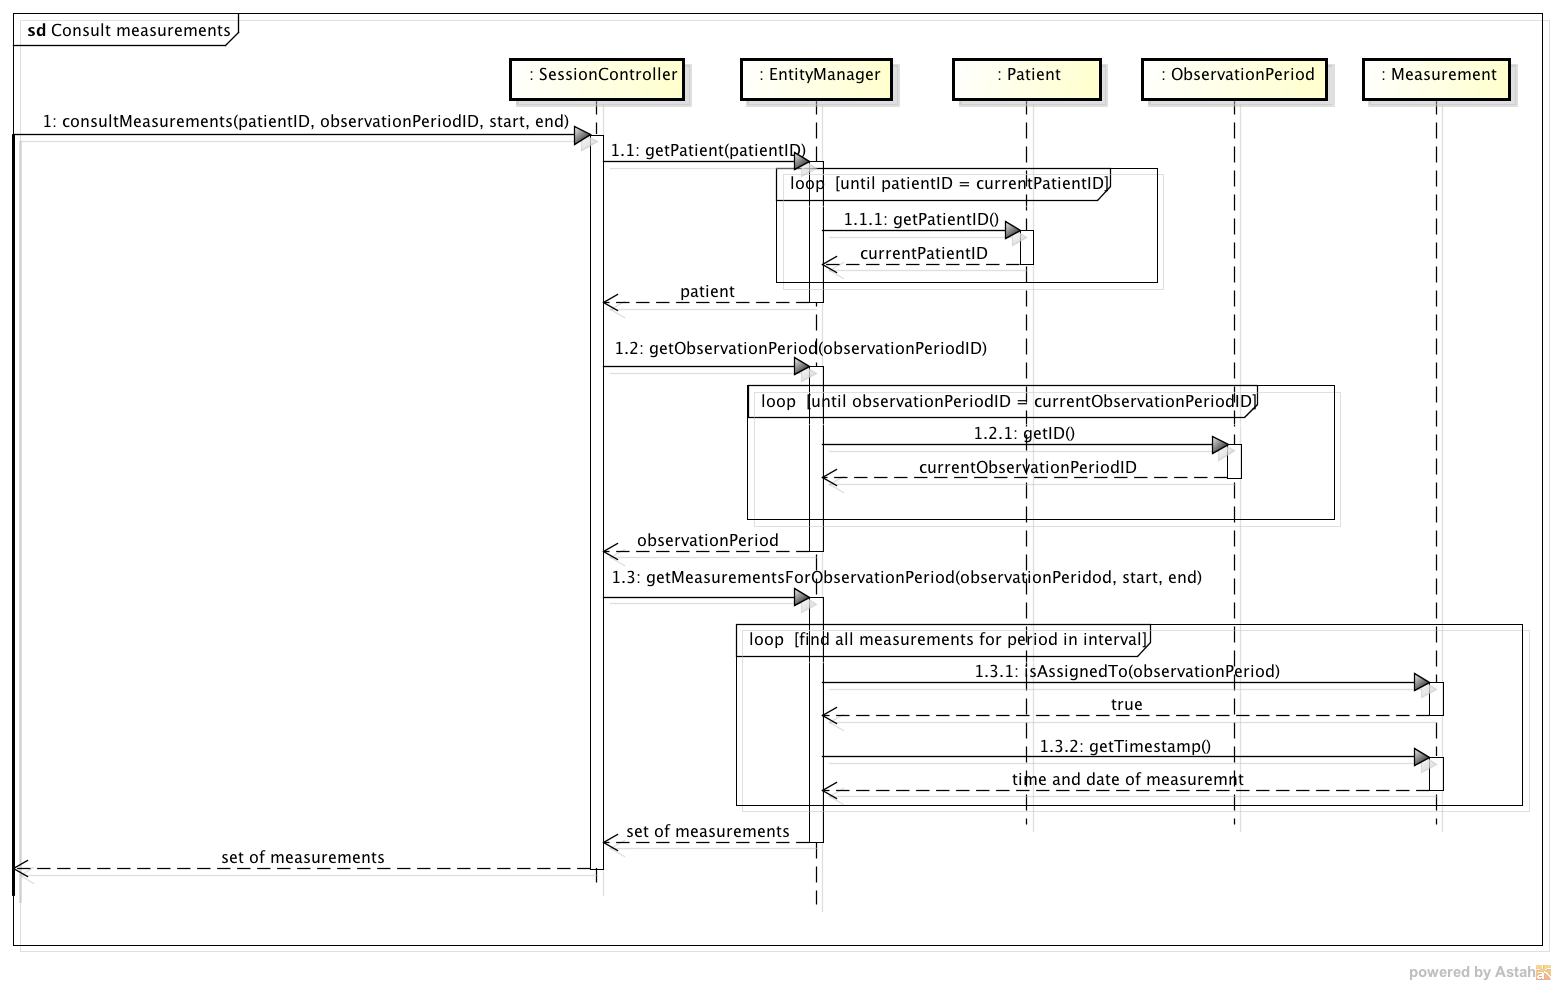
\includegraphics[width=15cm]{./img/sequence-diagrams/consult-measurements.png}

The SessionController first looks up the Patient, ObservationPeriod by querying the EntityManager and will then query the EntityManager for all Measurements concerning the given timespan in the ObservationPeriod.

\subsection{Design class diagram}


% Diagram generated with astah
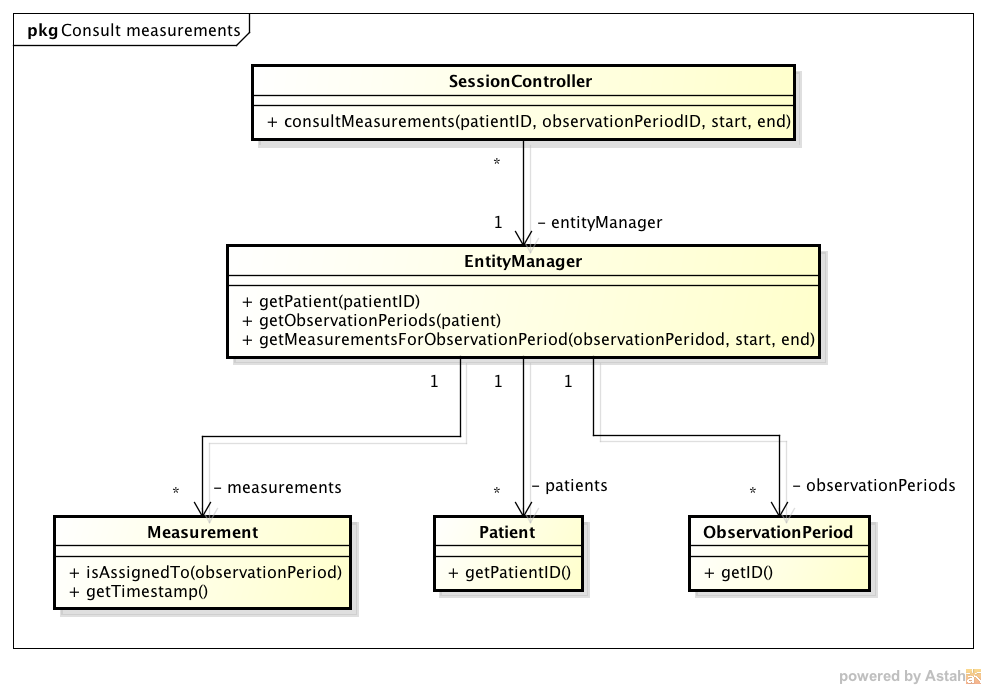
\includegraphics[width=15cm]{./img/design-class-diagrams/consult-measurements.png}

The SessionController queries the EntityManager for the desired measurements.

\section{Consult observation periods}

\subsection{System sequence diagram}

% Diagram generated with astah
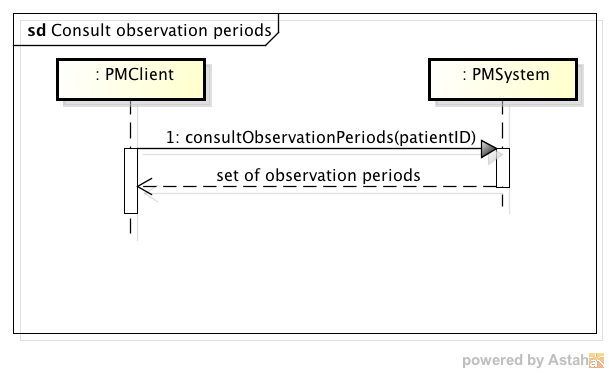
\includegraphics[width=10cm]{./img/system-sequence-diagrams/consult-observation-periods.png}

This diagram shows the communication between the client and the patient monitoring system. The patient invokes the method consultObservationPeriods with a patient's id and he gets a set of all observation periods which are assigned to him.

\subsection{Sequence diagram}

% Diagram generated with astah
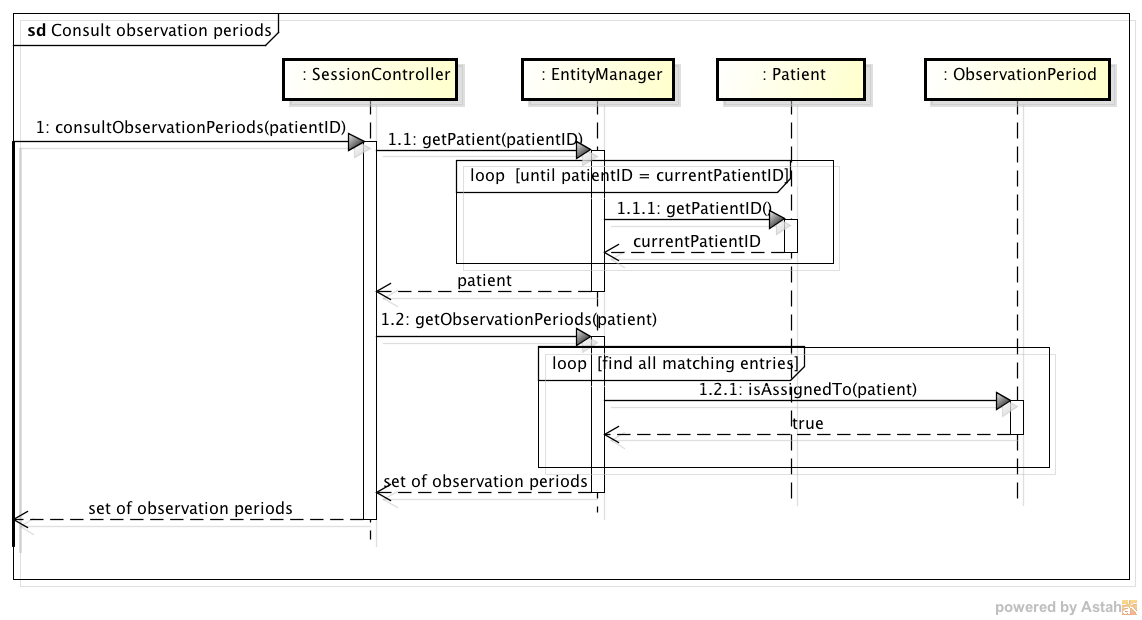
\includegraphics[width=15cm]{./img/sequence-diagrams/consult-observation-periods.png}

The SessionController looks up the Patient and then he will query the EntityManager for Observation Periods which are assigned to this Patient.

\subsection{Design class diagram}


% Diagram generated with astah
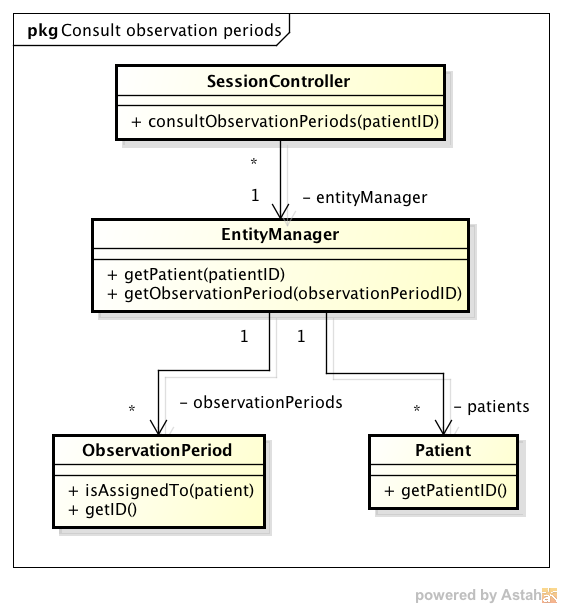
\includegraphics[width=10cm]{./img/design-class-diagrams/consult-observation-periods.png}

The SessionController accesses the Patient and the ObservationPeriods via the EntityManager. 

\section{Return device}

\subsection{System sequence diagram}

% Diagram generated with astah
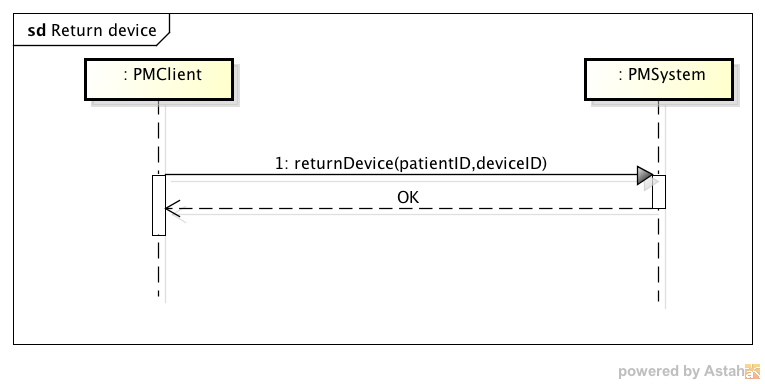
\includegraphics[width=10cm]{./img/system-sequence-diagrams/return-device.png}

For returning a device the client sends a message to the system which is acknowledged.

\subsection{Sequence diagram}

% Diagram generated with astah
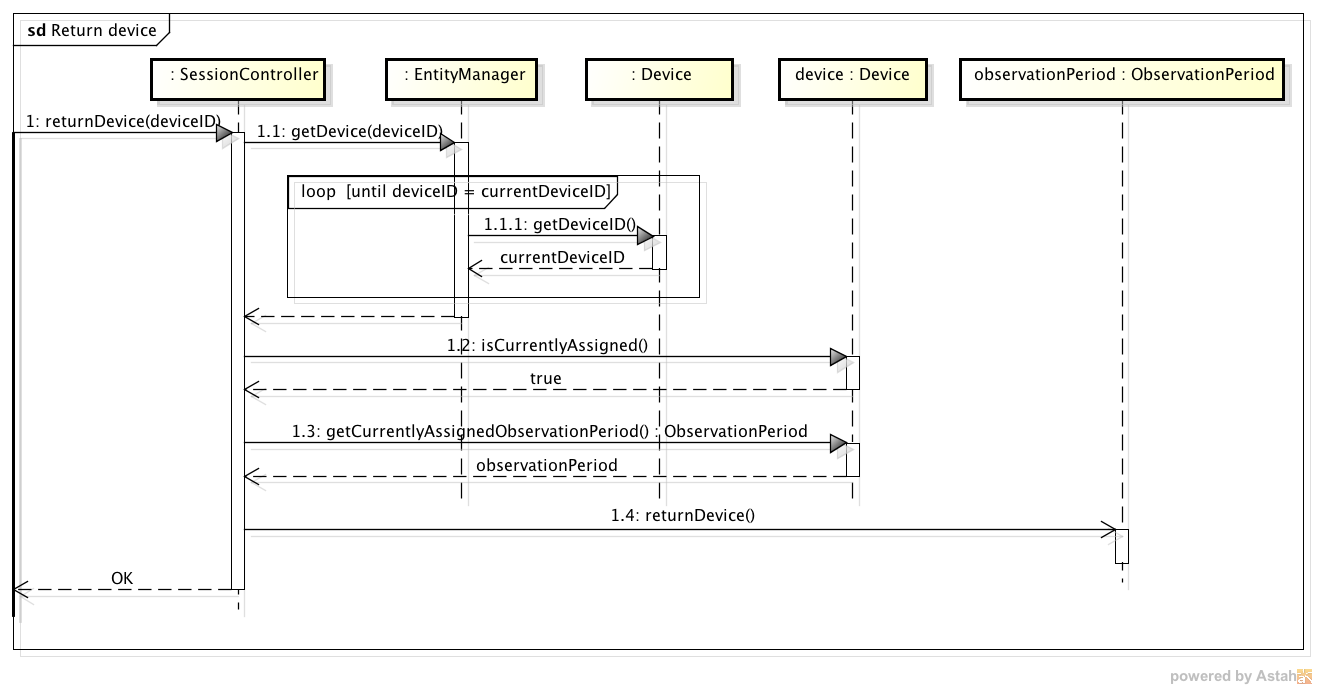
\includegraphics[width=15cm]{./img/sequence-diagrams/return-device.png}

For returning a device the session controller get the device from the entity manager. He checks if the device is actually assigned and gets the observation period from it. The returning of the device is then done on the observation period object.

\subsection{Design class diagram}

% Diagram generated with astah
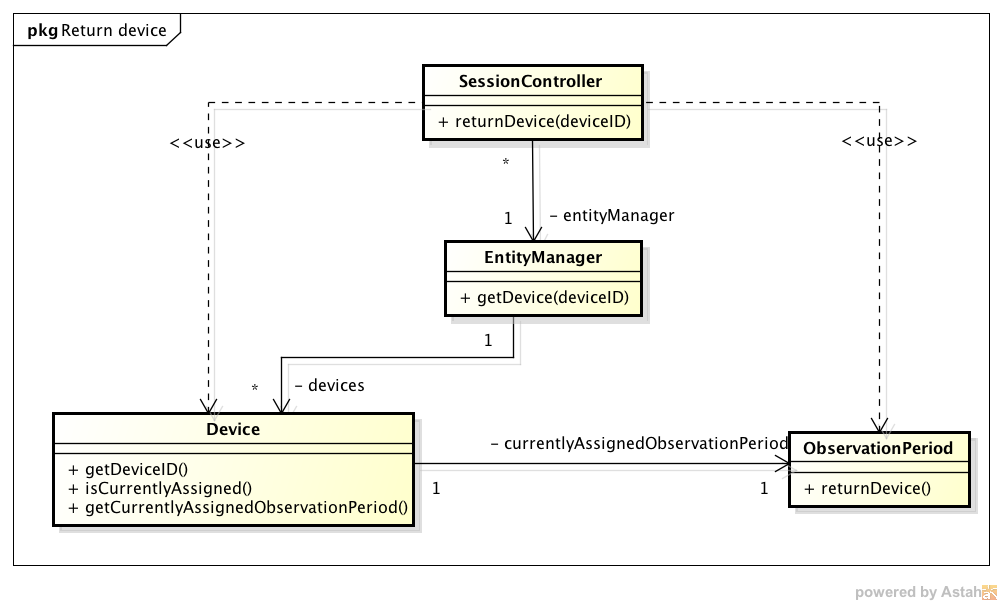
\includegraphics[width=15cm]{./img/design-class-diagrams/return-device.png}

The session controller uses the entity manager to get the device, from where it gets the observation period.

\end{document}